\documentclass[]{report}
\usepackage{url}
\usepackage{graphicx}
\usepackage{amsmath,amssymb}
\usepackage[numbers]{natbib}
\usepackage{titlesec}
\usepackage{appendix}
\usepackage{pdfpages}
\usepackage{verbatim}
\usepackage{titling}
\usepackage{lscape}
\usepackage[hidelinks]{hyperref}
\newcommand{\subtitle}[1]{%
	\posttitle{%
		\par\end{center}
	\begin{center}\large#1\end{center}
	\vskip0.5em}%
}

% Title Page
\title{KV6002 - Team Project and Professionalism}
\subtitle{Evaluation Report}
\author{Liam Brand}
\date{}

\begin{document}
\maketitle
\tableofcontents

\section{The System Produced}
The overall project aim was to develop a prototype system that involves several sensors monitoring an environment, and then using the data acquired from this for analytics and visualization through an appropriate medium. This section aims to explore the implemented features with regards to how well they were implemented according to various criteria.

	\subsection{Fitness for Purpose}
	Subsystems were successfully implemented to meet the overall project goal outlined earlier. Two sensors were developed that posted data to a database, and a front end containing appropriate functionality for data visualization and analysis was created as well. The visualization and analysis subsystems were also made capable of communication with both devices, allowing the system to communicate with multiple environmental sensors. The physical demo was proof of the product's functionality.
	\medskip
	
	As well, these elements have been implemented to be near real-time, as stored and processed data needs to be up to date for the system to be accurate. Analysing an hour old reading for example might not provide useful information as it's uncertain whether or not this reading represent the environment's current state. The sensors post their readings to the database every 15 seconds, allowing for the database to receive sensory data at a relatively quick pace. As well, XML http requests have been configured to fire every few seconds for relevant data visualization and data analysis methods, ensuring what is displayed or analysed is the most up to date information available and provides the most value to the user.
	\medskip
	
	Adherence to industry standards was also achieved where possible. For example, the model features an ability to inform users of problematic temperature differences between sensors. When discussing temperature differences between rooms, IBACOS - a strategic partner of the US Department of Energy - notes that "Room-to-room temperature differences or floor-to-floor temperature differences should be no greater than 4 degrees Fahrenheit in the heating season"\cite{burdick2011advanced}. The model therefore used this as a guide for its temperature difference threshold, but unknowns such as the temperature location, potential for sensory noise and use of only one sensor rather than one for each room, so the threshold was increased to four degrees celsius to accommodate for these aspects.
	
	\subsection{Robustness}
	AWS Lambda is used, which features functionality to allow scaling\cite{awslambdadocs} allowing the database to cope with additional device implementations. The devices themselves have features to cope with failures. It features two temperatures sensors with the second one being used if the first one fails, features in code to prevent erroneous measurements. As well, the devices will automatically attempt to reestablish internet connection upon being disconnected, and they also feature a 32GB Micro-SD card as temporary storage for readings data should connection be lost. Web elements such as the model's code contains try/catch statements to handle exceptions such as empty readings from the database as well, and will print appropriate messages to the console to assist in troubleshooting should these issues occur.
	
	\subsection{Look and Feel}
	Petrie and Fraser\cite{petrie2004tension} describe different issues that significantly impede users' ability to properly make use of a website. The primary offenders are complex pages, unclear navigation and poor colour contrast. The website's pages are simple, with large block elements for listed devices and clear headings denoting sections such as the model's device comparison results. Navigation is achieved via the use of a navbar, something seen often in websites and so it shouldn't be unfamiliar to users. The website's colour scheme is mainly dark blue and white, offering a good contrast between the background and elements like text. These aspects allow the system's interactive element to be familiar, easy to use and visually pleasing.
	\medskip
	
	The device could look better however. It's primarily made up of breadboards with components wired into them. Whilst functional, it doesn't look very visually appealing. Should it be deployed industrially, a more aesthetically pleasing case to house the components should be developed.
	
	\subsection{Consistency}
	Subsystems were developed with other subsystems in mind. For example, the website was properly formatted to make space for the data visualization and intelligent model. These elements have clear areas of the web page reserved for them that allows them to blend into the rest of the website, and they were included in the media queries to ensure they scaled to different screen sizes. The database endpoints allow the developed sensors to post data to the database, and endpoints were also created to provide the visualization and model subsystems with the data that they needed to perform their functions. These things allowed subsystems to work together without anything feeling like it wasn't accommodated for.
	
	\subsection{Technical Evaluation}
	Employed technology was appropriate for each subsystem. The devices used sensors that gathered relevant data, the database allowed the creation of needed endpoints and included inbuilt scaling technology, and the website subsystem's usage of HTML and CSS allowed for a pleasant looking website. The use of JavaScript for the visualization and model subsystems allowed for the creation of automated HTTP requests that ran every few seconds. This allowed for the regular retrieval of relevant data from the database which helped these systems be accurate as they always use the latest data available in the database, and as such the latest data from the sensor.
	\medskip
	
	Code featured appropriate comments, indentations and method/variable names to maximize code readability. Proper functional decomposition was done where appropriate too. For example in the model, part of determining an ideal temperature was to look at temperature readings from the same time for previous days. For this, timestamps needed to be created so readings made around these times could be searched for and retrieved. Creation of these timestamps was initially done in the \textit{checkTemperature} method, but it was later turned into a \textit{getPreviousTimestamps} helper function to maximize readability and group together relevant code.
	
	\subsection{Non-Functional Requirements}
	Primary non-functional requirements concerned the website's usability and the rate at which data was retrieved from the sensors and processed. These aspects have already been covered in previous sections. There is also a requirement for the development of an economic model to help cost the intelligent model, which can be viewed in Appendix B.

\section{Project Management, Process and Personal Achievement}
	\subsection{Terms of Reference}
	The description of subsystem requirements aided development by providing an understanding of the scope, complexity and methods/technologies that were used for their implementation. For example, the model's specification helped bring up some early questions regarding its possible behavior (e.g. what to do if it's too hot) and this allowed the developer to know what needed to be understood before development could begin. Discussion of the project's testing could have used more depth however, and things like unit testing (and perhaps the respective testing frameworks for the different technologies being used) could have been mentioned.
	
	\subsection{Requirements and Design Documentation}
	For requirements, a questionnaire was used with the client, shown in Appendix E, as well as numerous client meetings to fine tune requirements outlined from initial talks and the questionnaire. This consistent communication allowed for a high level view of the requirements to be understood, followed by understanding the requirements' finer details. Other products on the market were also reviewed, such as the ecobee4\cite{ecobee4} smart thermostat. This allowed an understanding of what the market already provided, helping determine some possible features to make the product more competitive on the marketplace.
	\medskip
	
	For design, wireframes for the website were created, shown in Appendix C. These helped in understanding how the website would look which helped development, and also allowed the data visualization and model subsystems to understand how their respective information should be output so that it can fit into the created website (e.g. how do we tell the user it's too hot in a way that displays well on the designed page?).
	
	\subsection{Time Management}
	Most time objectives were met, shown by the meeting minutes' satisfaction of a live end to end product by March. Development primarily finished mid April however rather than the start of April, so a more thorough understanding of task complexity and required development time is needed.
	
	\subsection{Configuration Management and Integration Strategies}
	Configuration and integration was primarily managed through the use of version control. A global repository was created with each group member added as a collaborator, and changes were committed and pushed to their own branches where appropriate. These branches were reviewed to determine their compatibility with existing code and merged into the master branch after. This ensured that all written code fit together without breaking other elements, and also provided a global repository accessible by each group member for the project's source code. Appendix A shows an excerpt of a git log, showing some of the commits, pull requests, and merges done to build the website. 
	
	Integration of subsystems was also discussed during meetings, for example the meeting on the 25th of March features an end to end prototype utilizing basic subsystem functionalities together. This enabled smaller iterative integrations rather than connecting everything all at once at the end and risking subsystems interfering with and breaking eachother.
	
	\subsection{Testing Strategies}
	Use of the project during code merges on git ensured that code updates didn't break the project, and a live end to end demo was conducted prior to the demonstration to ensure all features worked. A more thorough style of integration testing with a sophisticated testing plan would have been better however, and unit tests for specific code elements would have helped ensure system stability.
	
	\subsection{Group Leadership}
	No leader was elected among the group, this had issues in determining solid internal deadlines on different pieces of functionality. Likely this is one of the reasons that the project's time plan couldn't be properly adhered to.
	
	\subsection{Quality Planning}
	Group members inspected each others developed code to look for faults overlooked during initial development. These code reviews helped prevent tunnel vision where issues are repeatedly overlooked. To increase efficiency, notes could be made from these code reviews and published in a group folder for others to see, so they can check their own code during development for similar mistakes.
	
	\subsection{Potential Additional Functionality}
	As of right now the visualization and analysis subsystems are hard coded to only retrieve data from the two created devices, moving forward this should be made more dynamic to accommodate for additional created devices to allow these subsystems to function properly as more devices are added. In addition, the data visualization could be scaled up to display data from longer periods of time (e.g. months or years). Also, the data analysis is limited in what it does with the information it learns. For example if gas or an extremely high temperature is detected in a reading this manifests through website alerts, but a fully realised product could notify the appropriate services automatically to help the user. Important notifications could also be harder to miss, sending them to the users phone as a regular mobile notification. These aspects may have been achievable with better time management.
	
	\subsection{Problems Encountered, Their Solutions, and Lessons Learned}
	Better time management could have been achieved from sticking to the project plan, in future more attention will be paid to these time plans to prevent falling behind too much. Also, a better idea of whether or not to have a leader will allow more discipline in sticking to self imposed deadlined, so in future it would be better to explicitly discuss whether or not the group will have a leader and if so, who it is.

\section{Professional Issues}
The Code of Conduct was adhered to with good collaboration between teammates, as each member showed up to the group meetings and gave fair warning if other commitments would cause them to be late. Members were polite whilst still offering fair criticism. Moving forward these standards would need to be strictly adhered to, as insufficient communication between team members could cause project issues that directly affect clients causing a loss of faith in the company and as such the developed product.

\section{Legal Issues}
Data breaches against stored data were considered during the TOR. The usage of AWS helped mitigate this, with their databases featuring implemented security measured\cite{awsdatabasedocs} such as encryption and private keys required for endpoint access helping ensure the stored data is private. The repository containing the project's source code was also private with read and write privileges only given to group members, to prevent source code leaks. Terms of use such as copyright conditions were also adhered to, for example the AWS service terms\cite{awsserviceterms} were reviewed against proposed project functionality to ensure what we were using them for was acceptable by Amazon. These terms included things like ensuring the only data stored on the database was lawfully obtained by us, and these terms would need to be kept in mind once other users come into the picture should the product be deployed industrially. 
\medskip

As well, the Data Protection Act\cite{dataprotectionact2018} will need to be considered should the project be deployed. In particular, the Act states that a person has the right to find out what data relating to a person is stored by an organisation. Facilities to provide customers with this data if they request it should be set up. It also states data shouldn't be kept for longer than is needed, so it should be determined how long sensory data is required for the system's ideal function and then functionality should be in place to ensure data that is no longer needed is properly disposed of. 

\section{Social Issues}
The major social concern with this product noted in the TOr is the perception of it from the public. Devices inside of a person's house sending information about its status can make many uncomfortable. During their study into the reasoning of users behind using or not using smart sensors and their opinions on them, Lau et al\cite{lau2018alexa} have a participant who says "with smart speakers...I can avoid having it, so I’d really not, I don’t want another thing that could possibly violate my privacy". This was difficult to mitigate during development as industrial deployment of the product never happened, so it was impossible to determine how users felt about it being in their home.
\medskip

Should the product be deployed, the company needs to have complete transparency in how the sensors behave, what they store about people's homes, how this data is stored and how it is processed to provide system functionality such as the short term decision making. This could be in the form of an FAQ on the website, as well as a complete willingness to answer more specific question should users contact the company. Being open will help dissuade any negative perceptions of the sensors as customers will fully understand what the product is doing and why.

\section{Ethical Issues}
The main ethical concern identified for the project was misuse of sensor date. This was mitigated during development as to retrieve sensory data special keys are required, and these keys were only given to developers who needed certain endpoints for database access. This meant everyone only accessed the endpoints (and as such, the data) that they needed. With regards to the database itself, access was mainly restricted to the subsystem's developer.
\medskip

Should the product be deployed this policy will need to continue to be adhered to so that only those who actually need data will have access to it. If a larger company was established, data privilege levels should be assigned to employees that dictate what they have access to. These levels will be based on what data the employee will need access to in order to perform their job.

	\bibliographystyle{plainnat}
	\bibliography{papers}
	\newpage
	\begin{appendices}
		\chapter{Git Log}
		\label{appendix:gitlog}
		\verbatiminput{log.txt}
		\chapter{Economic Model}
		\label{appendix:economicmodel}
		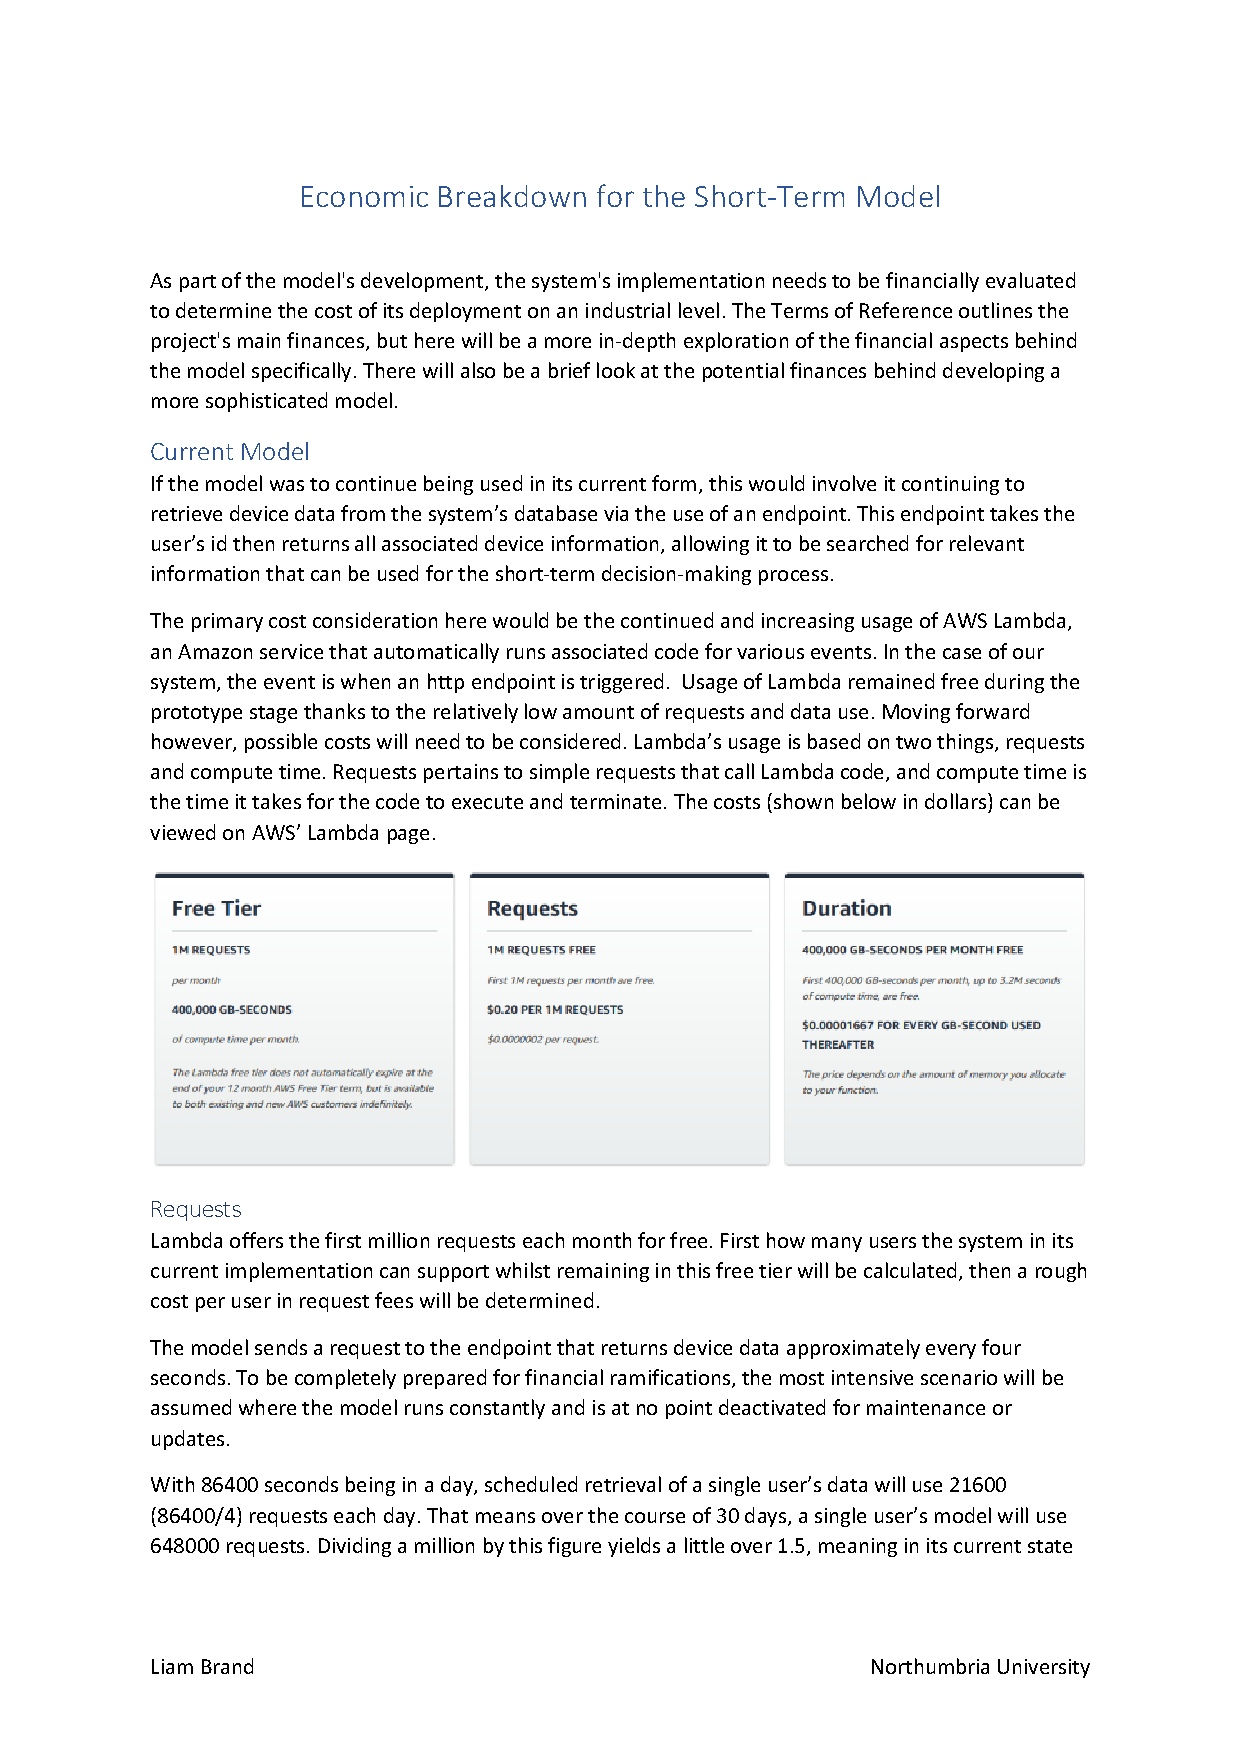
\includepdf[pages=-]{EconomicModel.pdf}
		\chapter{Wireframes}
		\label{appendix:wireframes}
		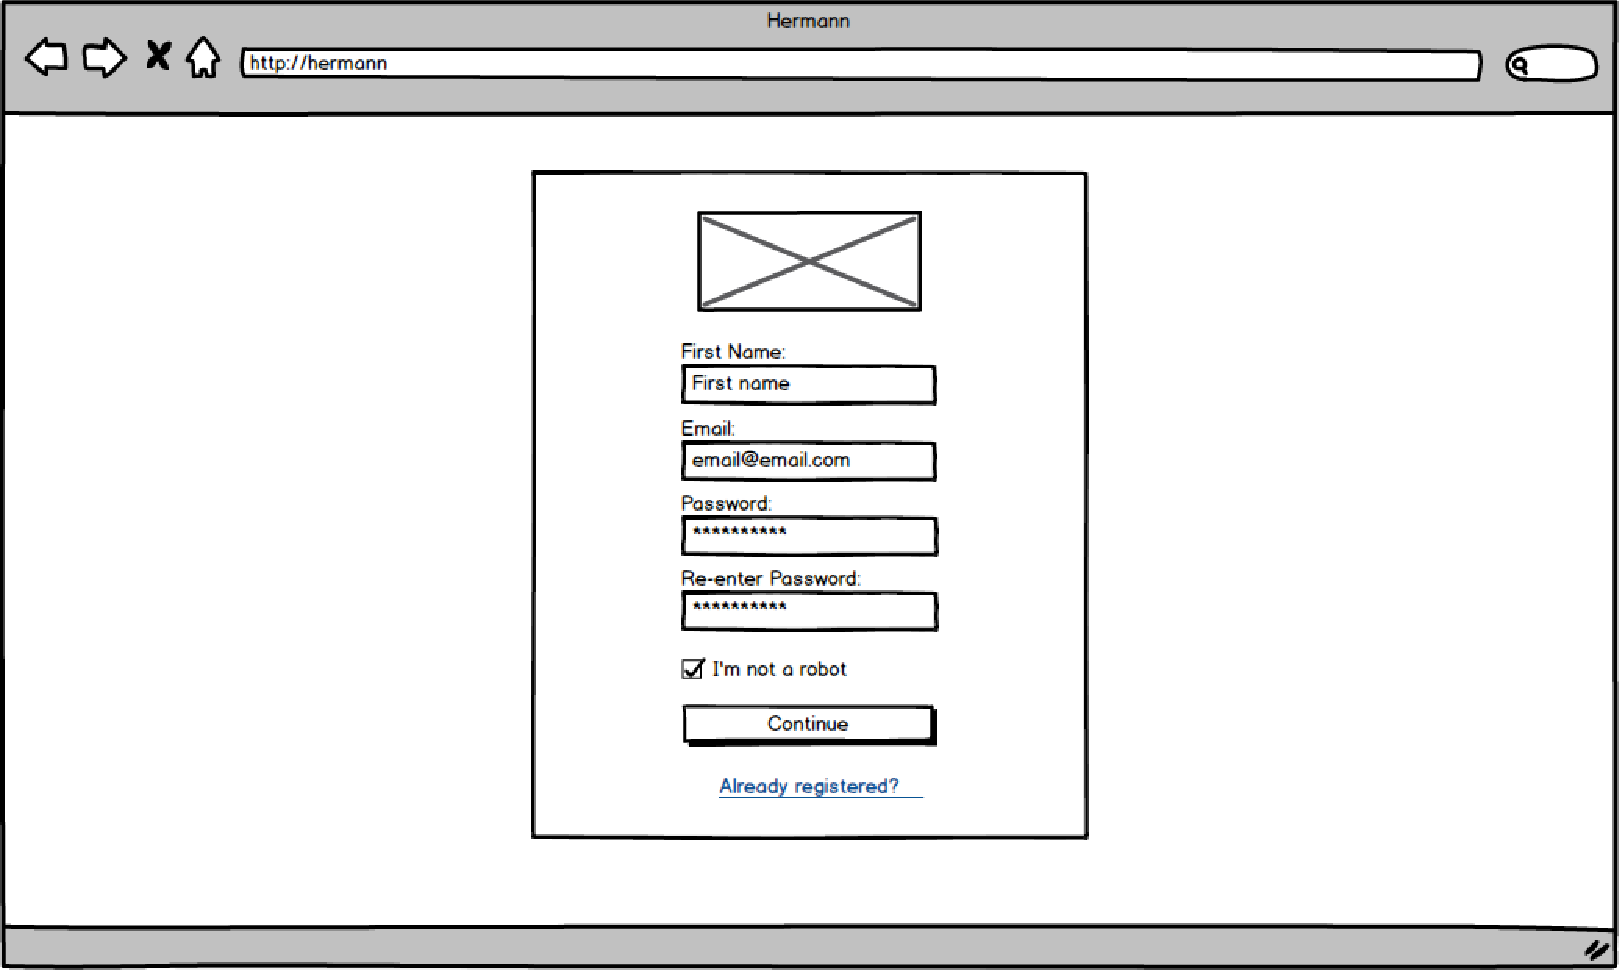
\includepdf[pages=-, landscape=true]{wireframes.pdf}
		\chapter{Infrastructure Diagram}
		\label{appendix:infrastructurediagram}
		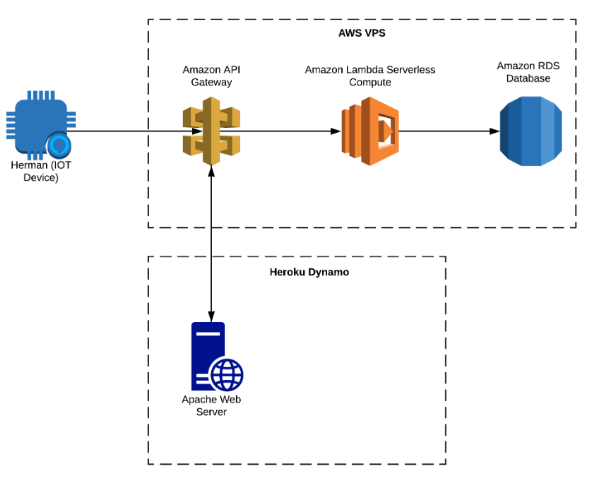
\includegraphics{awsmodel.png}
		\chapter{Client Questionnaire}
		\label{appendix:questionnaire}
		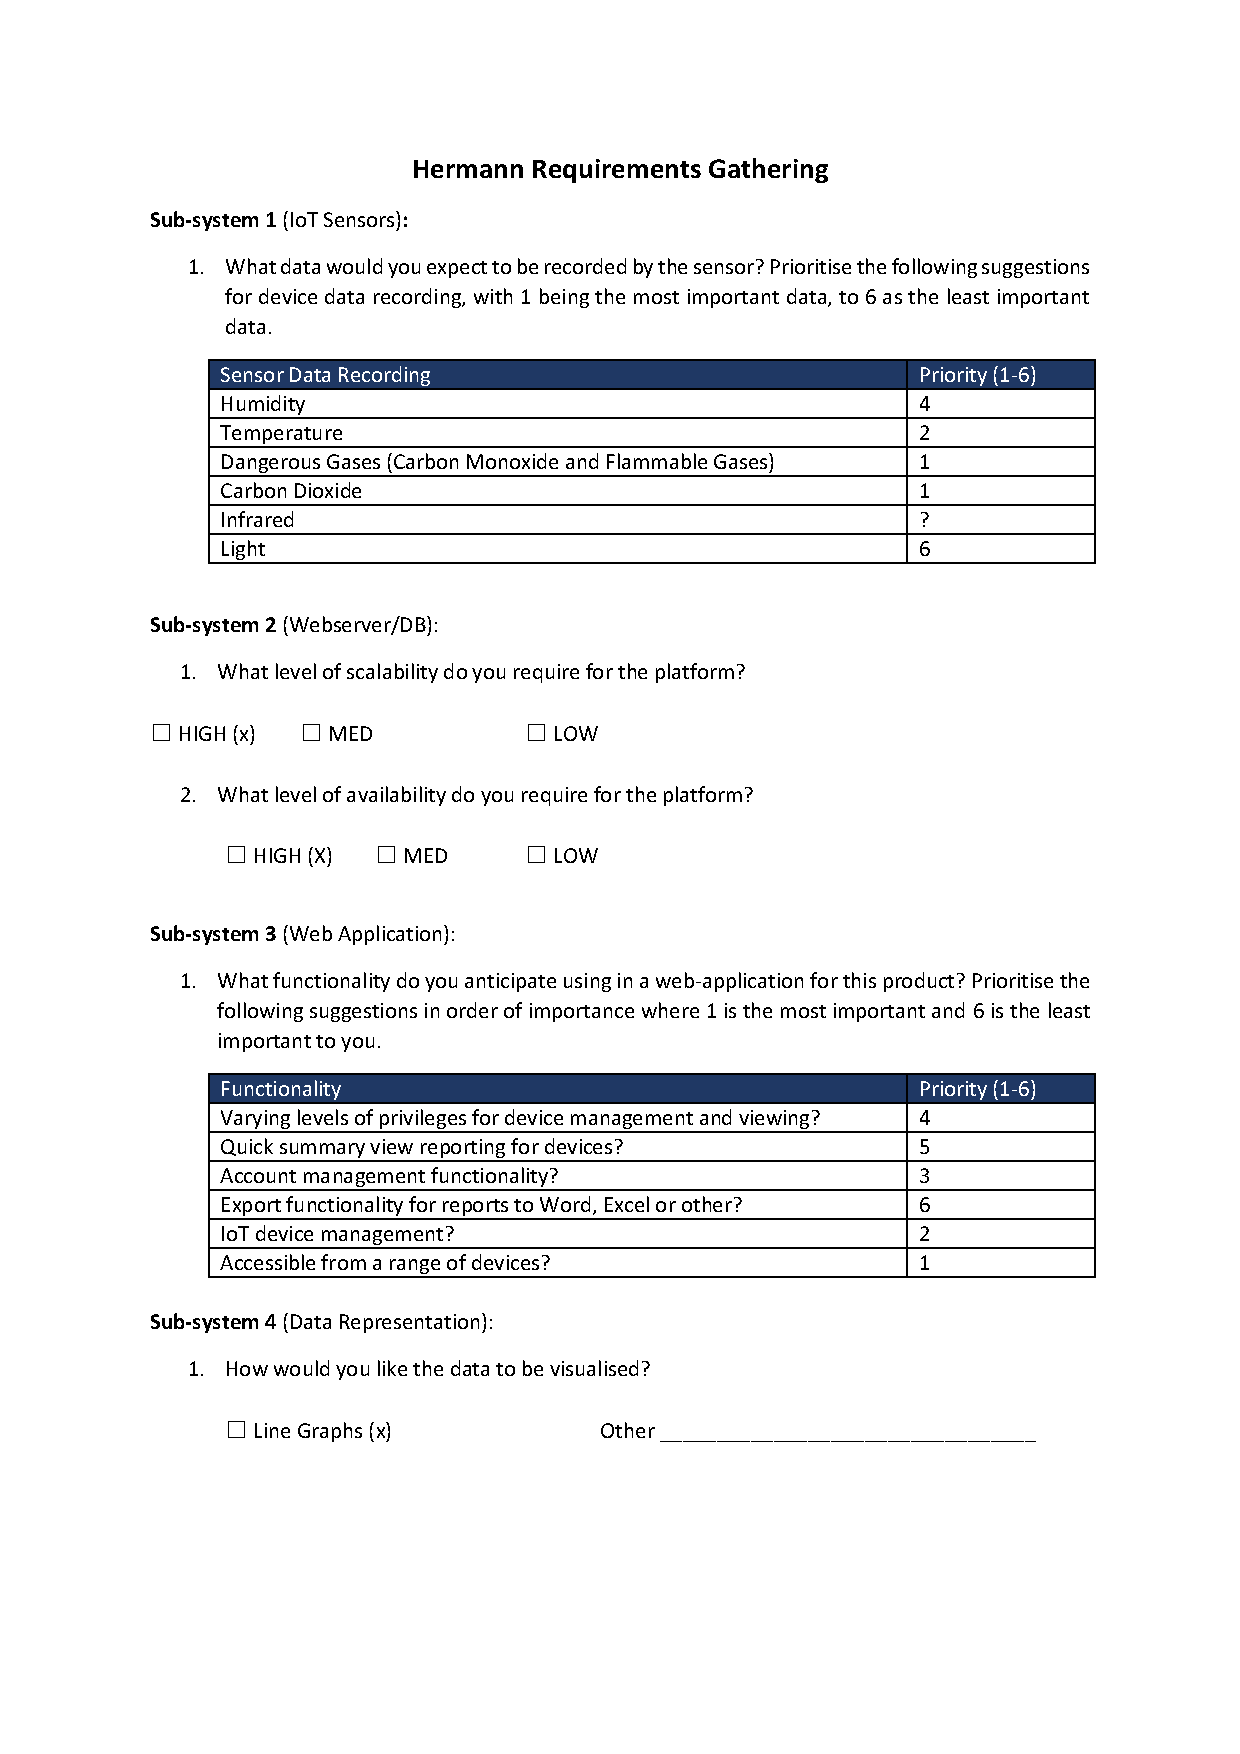
\includepdf[pages=-]{HUSEYIN-questionnaire.pdf}
		\chapter{Terms of Reference}
		\label{appendix:tor}
		
\includepdf[pages=-]{tor.pdf}
		\chapter{Meeting Minutes}
		\label{appendix:meetingsMinutes}
		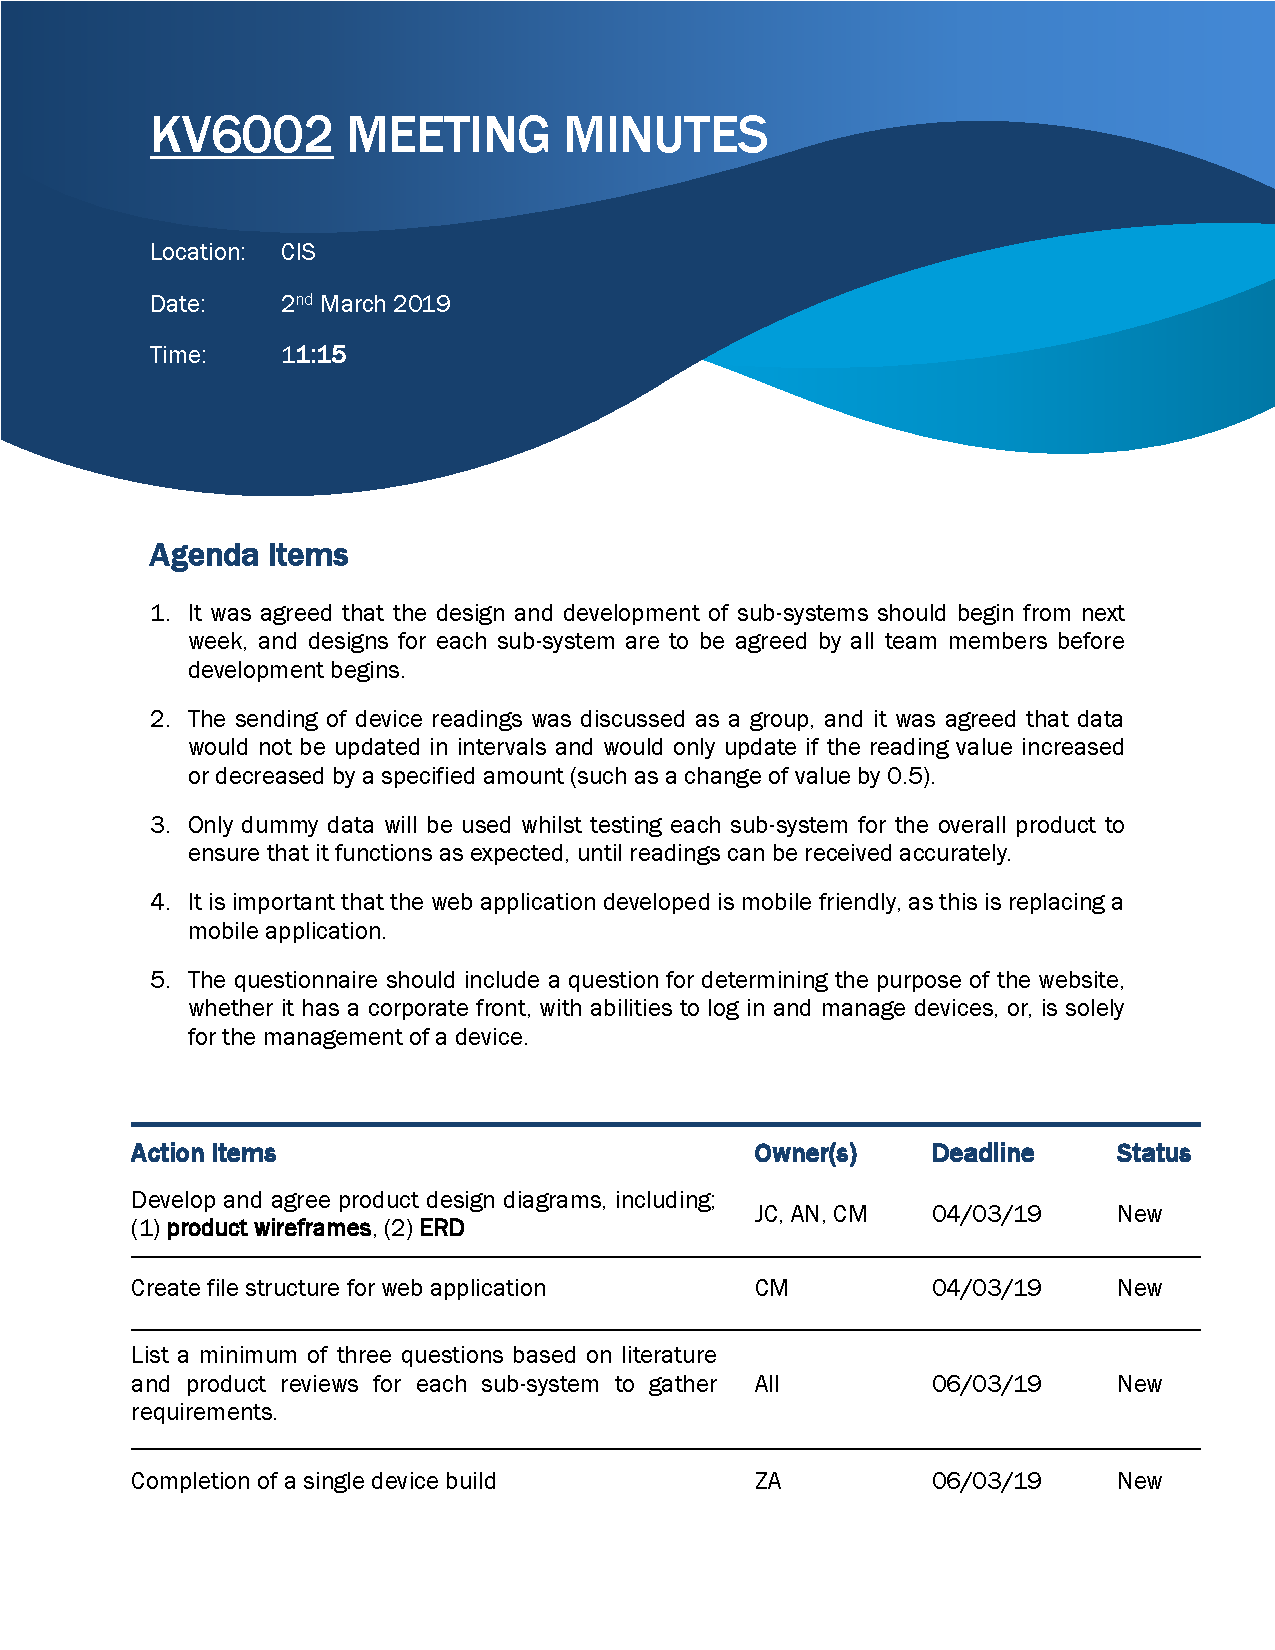
\includepdf[pages=-]{meetingminutes.pdf}
	\end{appendices}
\end{document}          
